

The results are shown in Table~\ref{tab:model_performance}. Overall, the evaluated models achieve modest extraction performance. For the primary location-impact metric, F1-scores range from 0.190 to 0.462. Gemini 3.5 Flash achieves the highest precision (0.469), recall (0.455), and F1-score (0.462), clearly outperforming the other evaluated models.

Claude Sonnet 4.5 achieves the second-highest recall, with a recall of 0.273 for the primary metric. This suggests that the model identifies relatively many drought impact events but also produces many false positives, resulting in a lower precision and overall F1-score. Despite being the most expensive model evaluated, Claude Sonnet 4.5 does not achieve the best overall extraction performance.

When the stricter location-impact-severity-recency metric is used, performance decreases substantially for every model. Gemini 3.5 Flash again achieves the highest performance with an F1-score of 0.185, while the remaining models score between 0.024 and 0.119. This indicates that correctly identifying a drought impact event is considerably easier than correctly extracting all associated event attributes.

One possible explanation for the strong performance of Gemini 3.5 Flash is that it is particularly well suited to structured information extraction tasks. Unlike complex reasoning benchmarks, this task primarily requires accurate entity extraction, classification, and structured JSON generation. Gemini Flash is designed for high-throughput structured workloads, which may better match the requirements of the proposed extraction framework. Another possible source of bias is that Gemini 3.5 Flash was used as a supporting tool during the manual annotation process. Although all annotations were manually verified, this may have introduced a small preference towards the model's output style.

Finally, the relatively low scores across all models are likely influenced by ambiguity in the impact taxonomy. During annotation, each event was assigned a single impact category, while multiple categories may reasonably describe the same drought impact. For example, an event describing reduced water availability for agriculture could potentially be labelled as irrigation shortage, water use restrictions, or reservoir and surface water shortage, depending on interpretation. Because the evaluation requires an exact category match, these semantic overlaps reduce the reported performance even when the extracted information is largely correct. This ambiguity is investigated further in the following sections.

\begin{table}[h!]
\centering
\caption{Event-level extraction performance of the evaluated LLMs.}
\label{tab:model_performance}
\small
\begin{tabular}{lccc|ccc}
\hline
& \multicolumn{3}{c|}{\textbf{Location + Impact}} & \multicolumn{3}{c}{\textbf{Location + Impact + Severity + Recency}} \\
\textbf{Model} & \textbf{P} & \textbf{R} & \textbf{F1} & \textbf{P} & \textbf{R} & \textbf{F1} \\
\hline
Gemini 3.5 Flash      & \textbf{0.469} & \textbf{0.455} & \textbf{0.462} & \textbf{0.188} & \textbf{0.182} & \textbf{0.185} \\
Gemini 3.1 Pro        & 0.206 & 0.212 & 0.209 & 0.118 & 0.121 & 0.119 \\
Claude Sonnet 4.5     & 0.191 & \textbf{0.273} & 0.225 & 0.064 & \textbf{0.091} & 0.075 \\
Gemini 3.1 Flash-Lite & 0.242 & 0.242 & 0.242 & 0.061 & 0.061 & 0.061 \\
GPT-5.4 mini          & 0.157 & 0.242 & 0.190 & 0.020 & 0.030 & 0.024 \\
\hline
\end{tabular}
\end{table}





\label{sec:variable_performance}


%\subsection{Extraction Performance Overview}

\subsection{Category Ambiguity and Granularity}

The low performance across all models can partly be explained by the structure of the impact taxonomy itself. To interpret these findings, we consider the concept of fuzzy categories from fuzzy set theory, introduced by Zadeh. Fuzzy set theory describes categories without clear boundaries, meaning that an element can partially belong to multiple categories simultaneously. This concept is particularly relevant for natural language, where concepts are often not strictly separated.

Initially, drought impacts can be grouped into broad categories, such as agricultural, hydrological, and socio-economic impacts. However, these categories overlap in practice. For example, reduced water availability can directly cause agricultural losses, meaning that the same drought event can reasonably belong to both hydrological and agricultural categories. This overlap is illustrated in Figure~\ref{fig:fuzzy_5sets}.

A natural expectation is that increasing the number of categories would reduce ambiguity by creating more specific definitions. However, increasing category granularity does not remove ambiguity. Instead, broad overlaps between major categories are replaced by more specific overlaps between closely related categories, as illustrated in Figure~\ref{fig:fuzzy_20sets}.

\begin{figure}[h!]
\centering

\begin{subfigure}{0.49\linewidth}
\centering
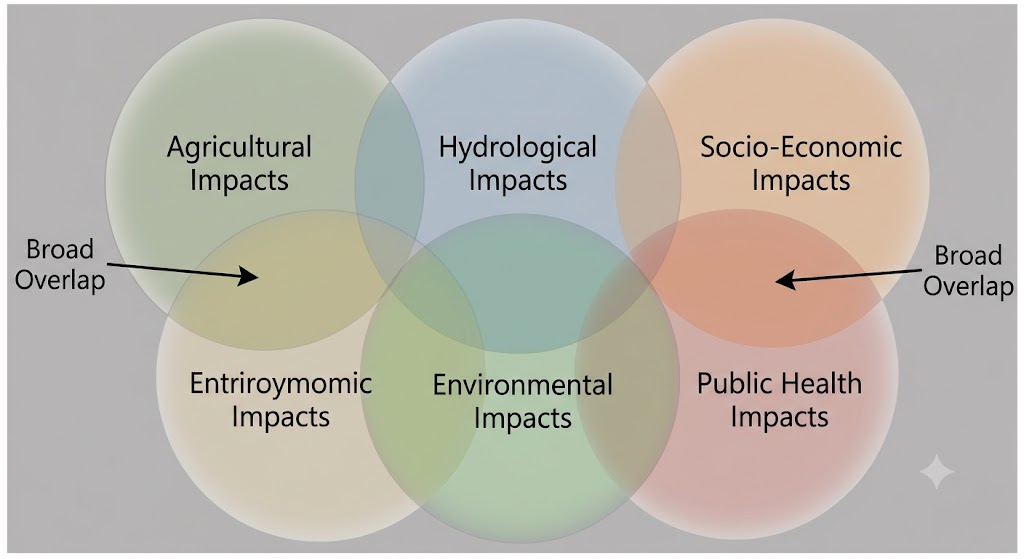
\includegraphics[width=\linewidth]{figures/Fuzzyset1.jpg}
\caption{Coarse-grained fuzzy impact categorisation (5 sets).}
\label{fig:fuzzy_5sets}
\end{subfigure}
\hfill
\begin{subfigure}{0.48\linewidth}
\centering
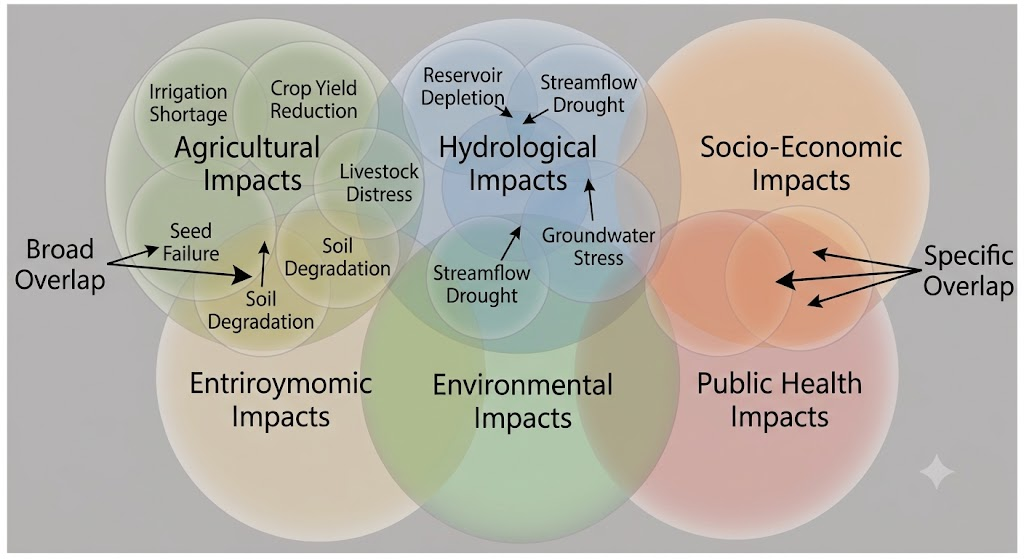
\includegraphics[width=\linewidth]{figures/Fuzzyset2.jpg}
\caption{Fine-grained fuzzy impact categorisation (20 sets).}
\label{fig:fuzzy_20sets}
\end{subfigure}

\caption{Comparison of coarse-grained and fine-grained fuzzy impact categorisations. Increasing category granularity changes the location of category overlap but does not remove ambiguity.}
\label{fig:fuzzy_comparison}
\end{figure}

For example, an article stating that farmers cannot irrigate because rivers have reached historically low water levels could reasonably be assigned to several categories, including irrigation shortage, reservoir and surface water shortage, water use restrictions, or agricultural impacts. However, annotation requires selecting a single ground-truth category. Therefore, a model prediction can be semantically correct while still being considered incorrect under strict evaluation.

This ambiguity is further increased by the event-level evaluation approach. A single drought impact may contain multiple related processes, but the evaluation requires an exact match between the predicted and annotated category. We attempted to account for this by allowing the model to extract multiple impacts for a single event, but in practice the model typically selected only the most dominant category.

\begin{figure}[h!]
\centering
\includegraphics[width=0.70\linewidth]{figures/Fuzzyset3.jpg}
\caption{Illustration of annotation ambiguity in the fine-grained impact categorisation.}
\label{fig:fuzzy_reality}
\end{figure}

Therefore, the relatively low extraction performance is not only caused by limitations of the language models but also by the difficulty of defining unique boundaries between drought impact categories. Figure~\ref{fig:fuzzy_reality} illustrates this challenge, where multiple categories can overlap for the same real-world drought impact. For example, the evaluation dataset contains many freshwater ecosystem degradation impacts, which could also reasonably be interpreted as surface water shortages in certain cases.

Future improvements could focus not only on improving model performance but also on developing annotation methods that allow multiple valid categories or different degrees of category membership.









\subsection{Post-hoc Evaluation and Structural Reformulation}

The previous evaluation showed that strict event-level matching can underestimate model performance when drought impacts have overlapping category boundaries. To further investigate this limitation, a post-hoc evaluation was performed on a subset of ten manually verified relevant articles. Instead of comparing predictions directly against a single ground-truth label, the extracted events were manually reviewed and classified as either correct, false positive, or false negative.

This evaluation provides a more direct assessment of whether the model identifies relevant drought impacts, independent of potential ambiguity in the predefined category labels. Therefore, it reduces the effect of strict category matching and allows us to distinguish between actual extraction errors and differences in interpretation between the model and the annotation.

In addition to the evaluation method, the extraction schema was reformulated to better represent the structure of drought impacts described in newspaper articles. The original formulation assumed that an article consists of multiple independent events, where each event represents a unique combination of location and impact category, together with additional attributes such as severity and recency. The model was therefore prompted to identify multiple events throughout the article.

However, this formulation does not fully reflect how drought impacts are commonly reported. A single location mention can describe several related impacts simultaneously. For example, an article discussing a drought-affected lake may mention reduced water levels, ecosystem degradation, and restrictions on water use at the same location.

The revised schema therefore follows a hierarchical structure. Instead of directly extracting independent events, the model first identifies location mentions and subsequently extracts all relevant impacts associated with each location. This formulation better represents the relationship between locations and impacts and reduces the need for the model to repeatedly search through the article for separate events.

The revised structure is:

\begin{itemize}
\item Article $\rightarrow$ Location mention
\item Location mention $\rightarrow$ Impact 1, Impact 2, Impact 3, ...
\item Each impact contains category, severity, recency, and supporting evidence
\end{itemize}

This reformulation is expected to improve the model's ability to identify multiple impacts associated with the same location and provides a more natural representation of drought impact reporting. The results of this post-hoc evaluation are presented in the following section.



